\documentclass{article}
\usepackage{amsmath}
\usepackage{graphicx}
\usepackage{fancyhdr}
\usepackage{array}
\usepackage{booktabs}
\usepackage[sorting=none]{biblatex}
\usepackage[margin=1in]{geometry}
\usepackage{listings}

\lstset{
    language=Python,                    % تنظیم زبان پایتون
    backgroundcolor=\color{white},      % رنگ پس‌زمینه سفید
    basicstyle=\ttfamily\footnotesize,  % استفاده از فونت monospaced
    keywordstyle=\color{blue},           % رنگ کلمات کلیدی
    commentstyle=\color{green},         % رنگ کامنت‌ها
    stringstyle=\color{red},            % رنگ رشته‌ها
    numbers=left,                       % شماره‌گذاری خطوط
    numberstyle=\tiny\color{gray},      % استایل شماره‌های خطوط
    stepnumber=1,                       % شماره‌گذاری هر خط
    numbersep=5pt,                      % فاصله شماره‌گذاری از کد
    showspaces=false,                   % نمایش فضاها
    showstringspaces=false,             % نمایش فضاها در رشته‌ها
    showtabs=false,                     % نمایش تب‌ها
    frame=single,                       % نمایش قاب دور کد
    rulecolor=\color{black},            % رنگ قاب دور کد
    tabsize=2,                          % اندازه تب‌ها
    captionpos=b,                       % عنوان در پایین قرار می‌گیرد
    breaklines=true,                    % تقسیم خط‌های طولانی
    breakatwhitespace=true              % تقسیم در فضای خالی
}
\usepackage[hidelinks]{hyperref}
\usepackage{subfigure}
\hypersetup{
    colorlinks=true,
    linkcolor=teal,
    filecolor=magenta,      
    urlcolor=teal,
    citecolor = teal
    }
\usepackage{xcolor}
\usepackage{xepersian}
\usepackage{fontspec}
\setlength\headheight{28pt} 
\addbibresource{bibliography.bib}
\settextfont[Scale=1.2]{IRLotus.TTF}
\setlatintextfont[Scale=1]{Times New Roman}
\renewcommand{\baselinestretch}{1.5}
\pagestyle{fancy}
\fancyhf{}
\rhead{
\includegraphics[width=1cm]{FaultD.png}مینی پروژه دوم درس یادگیری ماشین}
\lhead{\thepage}
\rfoot{امیر جهانگرد تکالو}
\lfoot{علیرضا امیری}
\renewcommand{\headrulewidth}{1pt}
\renewcommand{\footrulewidth}{1pt}
\AtBeginDocument{
	\def\chapterautorefname{فصل}%
	\def\sectionautorefname{پاسخ سوال}%
	\def\subsectionautorefname{بخش}%
	\def\subsubsectionautorefname{بخش}%
	\def\equationautorefname{رابطهٔ}%
    \def\lstlistingautorefname{برنامۀ}%
}
\renewcommand{\lstlistingname}{Code}
\begin{document}

\begin{titlepage}
\begin{center}

  \begin{figure}[h!]
 	\centering
 	\subfigure{
 		
\includegraphics[width=0.43\columnwidth]{KNTULogo.pdf}
 		\label{fig:FD3M4sav43i22ngCdW2}
 	}
 	\subfigure
 	{
 		
\includegraphics[width=0.33\columnwidth, height=0.45\columnwidth]{Fault}
 		\label{fig:FD3Msav43i22ngCdW2}
 	}
 \end{figure}
 
 % 
\includegraphics[width=0.5\textwidth]{KNTULogo.pdf}\\
 
\vfill
        
\Huge
\textbf{یادگیری ماشین}\\
\textbf{آزمون میان ترم}\\
        
\vfill
        
\begin{table}[ht]
    \centering
    \huge
    \begin{tabular}{|c|c|}
    \hline
    نام و نام خانوادگی & علیرضا امیری\\
    \hline
    شمارۀ دانشجویی &  40202414\\
    \hline
    تاریخ & خرداد ماه 1404\\
    \hline
    \end{tabular}
\end{table}
\end{center}
\end{titlepage}



\tableofcontents
\newpage


\section{پرسش 1}
\href{https://drive.google.com/drive/folders/1S5vMJYXH87PQ1vcxzW19rEgpDQKK5_Ni?usp=sharing}{لینک درایو گوگل کولب حاوی کدهای این تمرین}

\href{https://github.com/Alireza2001Amiri/KNTU-ML}{لینک Github}

\subsection{الف}
طبقه بندی بر اساس مدل بیز، یک روش مبتنی بر داده های آماری برای تفکیک کلاس های داده ها با در اختیار داشتن توزیع داده های هر کلاس می باشد. در تئوری، در صورت در اختیار داشتن توزیع دقیقی برای داده ها مطابق با معادلات حاکم بر بیز، می توانیم با بالاترین دقت دسته بندی را انجام دهیم. پیش از ادامه، معادله ی بیز را در رابطه ی زیر مشاهده می کنیم.

\begin{equation}
P(C_k | \mathbf{x}) = \frac{P(\mathbf{x} | C_k) \, P(C_k)}{P(\mathbf{x})}
\end{equation}

که در آن، 
\begin{itemize}
\item 
$C_k$ دسته ی $k$،
\item
$\mathbf{x}$ بردار ویژگی های رویت شده ی یک نمونه، 
\item
$P(C_k|\mathbf{x})$ خواسته ی مسئله که همان احتمال تعلق به دسته ی $K$ پس از مشاهده ی ویژگی های $x$ ،
\item
$P(\mathbf{x}|C_k)$ توزیع احتمال ویژگی ها در دسته ی $k$,
\item
$P(C_k)$ توزیع داده های دسته ی k,
\item
و $P(\mathbf{x})$ توزیع کلی تمام داده ها است.
\end{itemize}

بر اساس این رابطه، در صورت در اختیار داشتن تعدا بی نهایت داده، می توانیم احتمال تعلق داده های جدید به هر کلاس را به صورت قطعی محاسبه کرده و کلاسی که بیشترین احتمال را دارد به عنوان پاسخ قطعی انتخاب کنیم. بر اساس دانش آماری موجود در این روش، می توان دریافت که همواره در صورت برقرار بودن مفروضات این رابطه، پاسخ به دست آمده از آن بهینه خواهد بود. بر این مبنا، روش طبقه بندی بیز بهینه به صورت زیر مطرح می شود:
\begin{quote}
        پیدا کردن کلاس $C^*$ به گونه ای که $C^* = \arg\max_{C_k} P(C_k | \mathbf{x})$
\end{quote}
با این حال، محاسبه ی مقدار فوق مستلزم دانستن $P(\mathbf{x}|C_k)$ و $P(C_k)$ می باشد که در واقعیت امکان پذیر نیست.

برای فائق آمدن بر این مشکل و ساده سازی معادلات، در روش طبقه بندی بر اساس بیز ساده فرض می شود که ویژگی ها همه مستقل از یکدیگر هستند. بنابراین خواهیم داشت:
\begin{equation}
    P(\mathbf{x} | C_k) = \prod_{i=1}^{n} P(x_i | C_k)
\end{equation}
 آنگاه رابطه ی بیز به صورت زیر تقریب زده می شود:
 \begin{equation}
     P(C_k | \mathbf{x}) \propto P(C_k) \prod_{i=1}^n P(x_i | C_k)
 \end{equation}
و در روش طبقه بندی مطابق با هدف زیر تلاش می کنیم:
\begin{equation}
    C^* = \arg\max_{C_k} \left( P(C_k) \prod_{i=1}^n P(x_i | C_k) \right)
\end{equation}

بدین ترتیب، علی رغم فرض اشتباهی که در این رابطه در نظر گرفته شده است، می توانیم با در اختیار داشتن داده های محدود، با دقت مناسبی طبقه بندی را انجام دهیم. علاوه بر این، به دلیل ساده سازی های مفروض در این روش، generalization بیشتری نیز به دست خواهیم آورد.

\subsection{ب}
از میان انواع مختلف پیاده سازی های روش طبقه بندی بیز، در اینجا به بررسی سه روش Gaussian, Bernoulli و multinomial می پردازیم.

به طور مختصر، روابط ریاضی هر یک به شرح زیر است:
\begin{itemize}
    \item \textit{multinomial}
    \[ P(\mathbf{x} | C_k) = \frac{(\sum_i x_i)!}{\prod_i x_i!} \prod_{i=1}^n p_{ki}^{x_i}
    \]
    که در آن 
    $p_{ki}$
    توزیع احتمال کلمه ی iام در کلاس k است

    \item \textit{Bernoulli}
    \[
    P(\mathbf{x} | C_k) = \prod_{i=1}^n p_{ki}^{x_i} (1-p_{ki})^{1-x_i} 
    \]
        که در آن 
    $p_{ki}$
    توزیع احتمال وجود داشتن کلمه ی iام در کلاس k است

    \item \textit{Gaussian}
    \[
    P(x_i | C_k) = \frac{1}{\sqrt{2\pi \sigma_{ki}^2}} \exp\left( -\frac{(x_i - \mu_{ki})^2}{2\sigma_{ki}^2} \right)
    \]
        که در آن 
        $\mu_{ki}$ میانگین ویژگی i در کلاس k
        و 
        $\sigma_{ki}^2$ واریانس ویژگی i در کلاس k است.
\end{itemize}

بر این اساس، همان طور که در پروژه های انجام شده بر روی این دیتاست می توان مشاهده کرد، غالبا از روش multinomial استفاده شده است، از آنجا که در این روش، نه تنها حضور داشتن یا نداشتن، بلکه تعداد حضور کلمات در متن پیامک لحاظ شده است که در مقایسه با روش برنولی، مناسب تر به نظر می رسد. علاوه بر این، استفاده از روشی گوسی در مواقعی مناسب است که داده ها دارای مقادیر پیوسته باشند که در مورد این دیتاست قابل پیاده سازی نیست.

\subsection{ج. پیاده سازی مدل طبقه بندی به صورت دستی}
چنان که در بخش قبل نتیجه گیری شد، پیاده سازی مدل multinomial 
به عنوان مدل بهینه ی طبقه بندی برای دیتاست Spam که دارای محتوای حروف می باشد برای پیاده سازی انتخاب شده است. 
در این بخش، به پیاده سازی این مدل بدون استفاده از پکیج های موجود خواهیم پرداخت.

\subsubsection{بارگذاری دیتاست}
در بخش اول، دیتاست را با استفاده از کتابخانه ی pandas داخل محیط پایتون بارگذاری کرده و داده های ابتدایی آن را مشاهده می کنیم. (\autoref{fig:1})
\begin{figure}[h!]
    \centering
    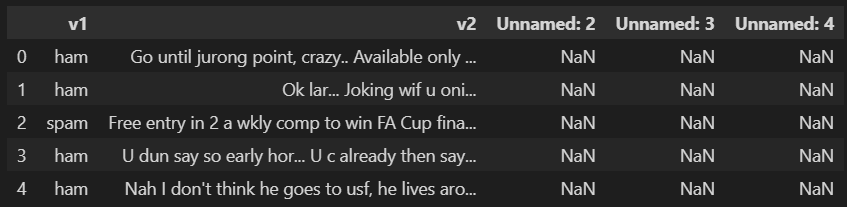
\includegraphics[width=0.5\linewidth]{1.png}
    \caption{ساختار دیتاست خام}
    \label{fig:1}
\end{figure}
\clearpage
با بررسی این ساختار، متوجه می شویم که برچسب های دیتاست در ستون اول و محتوای پیام ها در ستون دوم قرار گرفته است. علاوه بر این، تعداد 50 نمونه نیز در ستون ستوم دارای محتوای متنی هستند که از آنها صرف نظر کرده و حذف شان می کنیم.
در پایان، پس از نام گذاری ستون ها و حذف مقادیر نامعتبر NaN، دیتافریم به صورت نمایش داده شده در شکل \autoref{fig:2} به دست می آید.
\begin{figure}[h!]
    \centering
    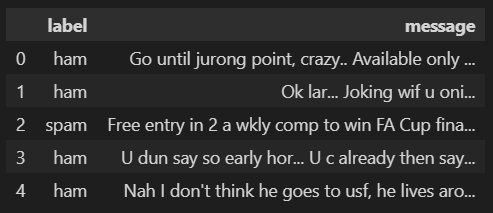
\includegraphics[width=0.75\linewidth]{2.png}
    \caption{دیتافریم اصلاح شده}
    \label{fig:2}
\end{figure}
\clearpage


\subsubsection{پیش پردازش}
تا به اینجا، دیتاست شامل داده های پیام ها و برچسب ها مشخص شده اند. با این حال، برای استفاده در مدل های یادگیری ماشین، لازم است داده ها از حالت حروف خارج شده و شامل محتوای عددی باشند.

برای این منظور، در طی چند مرحله متن ها را به محتوای عددی تبدیل می کنیم.
\begin{enumerate}
    \item \textbf{فیلتر کردن متن ها}
    
    در ابتدا، برای خالص سازی متن های موجود، نیاز داریم تا کلمات موجود در آنها را از فیلتر هایی بگذرانیم. برای این منظور با استفاده از پکیج NLTK
    به انتخاب و حذف این عوامل می پردازیم.
    \begin{itemize}
        \item حذف کاراکتر های خاص مانند $!@$
        \item کوچک کردن تمامی حروف
        \item حذف عبارات پرکاربرد مانند The, and, is
    \end{itemize}
    \item \textbf{تغییر برچسب های متنی به عددی}
    
    در اینجا، برچسب ها را به صورت زیر تغییر می دهیم و نگاشت می کنیم.
    $
\text{label} =
\begin{cases}
0 & \text{if } \text{label} = \text{"ham"} \\
1 & \text{if } \text{label} = \text{"spam"}
\end{cases}
$
\item \textbf{توکن بندی}

در این بخش که گامی مهم در پیش پردازش دادگان و استخراج ویژگی است، کلمات مورد استفاده در متن پیام ها به صورت عددی مطابق آنچه که پس از این توضیح داده می شود تبدیل می شوند. 
برای این منظور، از روش CountVectorizer در پکیج Sklearn استفاده می شود.
این روش، به هر کلمه که به عنوان ورودی داده می شود، یک توکن ثبت کرده و در نهایت لغت نامه ای شامل تمام کلماتی که با آن آموزش دیده است ایجاد می کند. زین پس، با دریافت هر جمله یا متن، با شمردن تعداد حضور هر کلمه در متن، عددی را برای توکن متناظر قرار می دهد که ما می توانیم از این توکن ها به عنوان ویژگی ها برای آموزش مدل استفاده کنیم.

پیش از اجرای این مرحله، لازم به ذکر است که برای جلوگیری از نشت اطلاعات از داده های Train به داده های Test، ما تنها می توانیم فرایند tokenization را بر روی داده های Train انجام دهیم و سپس به داده های Test منتقل کنیم. 
بنابراین، ابتدا داده ها را به دو دسته ی آموزش و تست تقسیم کرده و سپس vectorizer را بر روی آن آموزش می دهیم.

\end{enumerate}
در پایان این مرحله، داده های تست و آموزش به صورت نمایش داده شده در 
\autoref{fig:3}
به دست می آیند.
\begin{figure}
    \centering
    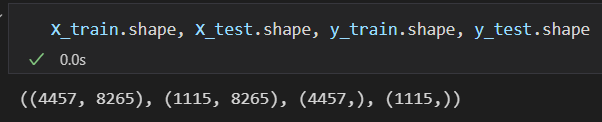
\includegraphics[width=0.75\linewidth]{3.png}
    \caption{داده های تست و آموزش پس از پیش پردازش}
    \label{fig:3}
\end{figure}
\clearpage

\subsubsection{آموزش مدل MultiNB به صورت دستی}
به منظور پیاده سازی دستی این کد، کلاسی به عنوان MultiNB تعریف می شود که در ادامه به توضیح روش های آن خواهیم پرداخت:
\begin{itemize}
    \item \textbf{prior} 
    
    در این کلاس، مطابق رابطه ی زیر، مقدار احتمال پیشین هر دسته به صورت زیر محاسبه می شود.
    \begin{equation}
        P(y = c) = \frac{\text{count}(y = c)}{n_{\text{samples}}}
    \end{equation}
    
    \item \textbf{fit}
    
    در این روش، به ازای هر کلاس مجموع تعداد هر ویژگی و مجموع تمام ویژگی ها در هر کلاس به صورت زیر به دست می آید.
    \begin{equation}
        N_{c,i} = \sum_{x \in D_c} x_i \qquad \text{and} \qquad N_c = \sum_i N_{c,i}
    \end{equation}

    \item \textbf{theta}

    در این بخش، تابع مشابهت likelihood داده های هر کلاس مطابق رابطه ی زیر محاسبه می شود.
        \begin{equation}
        \theta_{c,i} = P(x_i \mid y = c) = \frac{N_{c,i} + \alpha}{N_c + \alpha \cdot d}
    \end{equation}

    آنگاه با فرض استقلال ویژگی ها از یکدیگر، توزیع احتمال هر کلاس به صورت زیر محاسبه می شود.
        \begin{equation}
        P(\mathbf{x} \mid y = c) = \prod_{i=1}^{d} \theta_{c,i}^{x_i}
        \end{equation}

    لازم به ذکر است که در این روابط، از مقدار 
    $\alpha$ برای جلوگیری از بروز خطا در شرایطی که داده های موجود در دیتاهای تستی در توکن های آموزش دیده وجود نداشته باشند قرار داده شده است.

    \item \textbf{predict}

    در نهایت در این روش، احتمال پسین، یعنی احتمال تعلق داشتن به هر دسته، با فرض در اختیار داشتن ماتریس ویزگی ها را محاسبه کرده و در نهایت، کلاسی با بیشترین احتمال را به عنوان خروجی اعلام می کنیم. رابطه ی احتمال در این بخش از کد به صورت زیر محاسبه می شود.
    \begin{equation}
        P(y = c \mid \mathbf{x}) = \frac{P(y = c) \cdot P(\mathbf{x} \mid y = c)}{\sum_{c'} P(y = c') \cdot P(\mathbf{x} \mid y = c')}
    \end{equation}
    \begin{equation}
        \hat{y} = \arg\max_c \; P(y = c \mid \mathbf{x})
    \end{equation}
\end{itemize}

\subsubsection{آموزش مدل}
با تعریف مدل در بخش قبل، می توانیم به پیاده سازی آن بر روی دیتاست بپردازیم. 
پس از آموزش مدل با دستور fit و آزمودن مدل بر داده های تستی خواهیم داشت:\autoref{fig:4}

\begin{figure}
    \centering
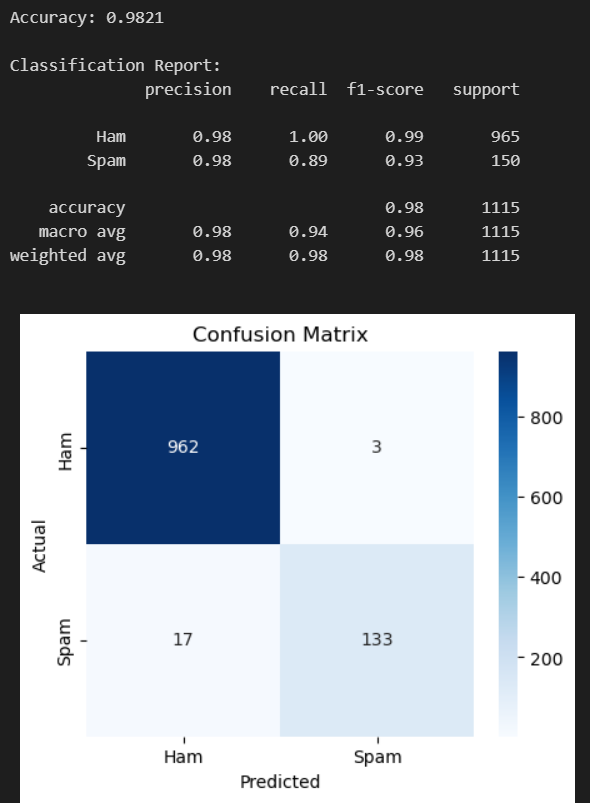
\includegraphics[width=1\linewidth]{4.png}
    \caption{گزارش طبقه بندی برای مدل MultiNB دستی}
    \label{fig:4}
\end{figure}
\clearpage

\subsection{د. پیاده سازی دو مدل طبقه بندی با استفاده از sklearn}

با در اختیار داشتن دیتاست چنان که در بخش پیشین توضیح داده شد، می توان مدل های دیگری از کتابخانه ی sklearn را بر روی داده ها آموزش داد. در اینجا، دو مدل MultinomialNB و ComplementNB انتخاب شده و داده ها بر اساس آن آموزش داده می شوند. 
گزارش طبقه بندی این مدل ها به شرح زیر خواهد بود. \autoref{fig:5} , \autoref{fig:6}
\begin{figure}
    \centering
    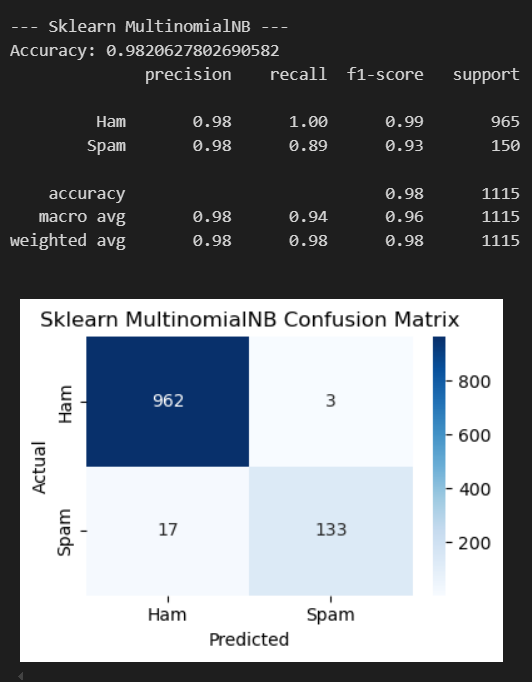
\includegraphics[width=0.75\linewidth]{5.png}
    \caption{گزارش طبقه بندی مدل MultiNB با استفاده از sklearn}
    \label{fig:5}
\end{figure}
\begin{figure}[h!]
    \centering
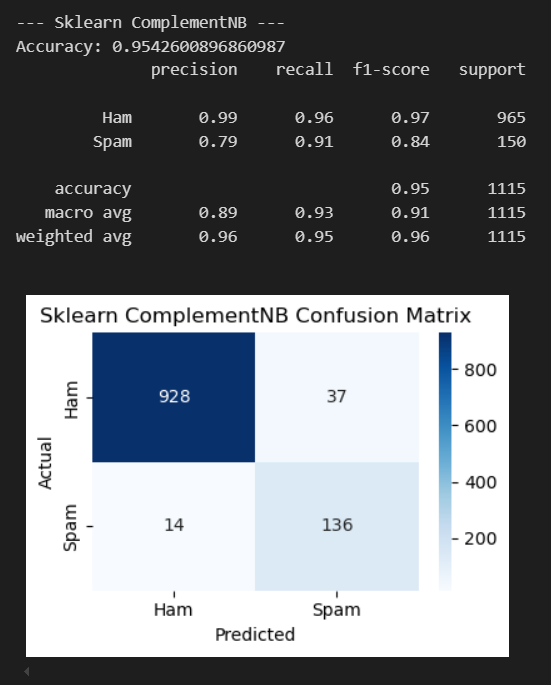
\includegraphics[width=0.75\linewidth]{6.png}
    \caption{گزارش طبقه بندی مدل ComplementNB با استفاده از sklearn}
    \label{fig:6}
\end{figure}
\clearpage
پس از این، برای مقایسه ی عملکرد مئدل ها با یکدیگر خواهیم داشت. \autoref{fig:7}
\begin{figure}
    \centering
    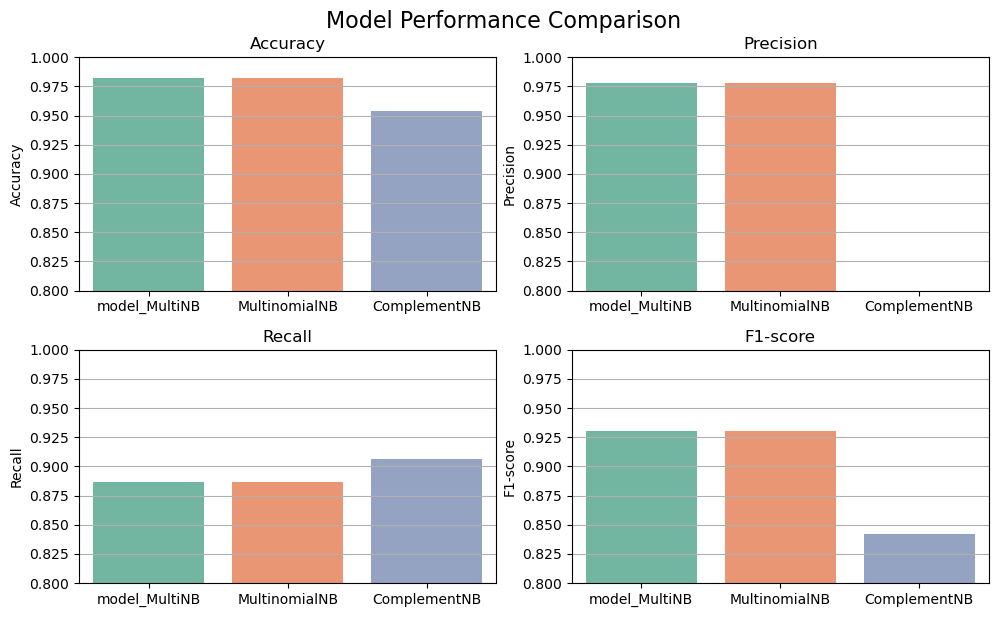
\includegraphics[width=0.75\linewidth]{7.png}
    \caption{مقایسه عملکرد مدل ها}
    \label{fig:7}
\end{figure}

از مقایسه این داده ها و بررسی پارامتر های گزارش شده، در می یابیم که اگرچه مدل ComplementNB دارای امتیاز recall بیشتری است، اما دقت آن در تشحیص پیام های spam تنها 70 درصد است که نشان می دهد این مدل توانسته spam های بیشتری را تشخیص دهد، اما با قیمت اینکه تعداد بسیار بیشتری از تایپ های ham را نیز به عنوان spam تشخیص داده باشد.
به غیر از این، دو مدل دیگر که مربوط به multiNB هستند عملکرد یکسانی دارند و این نشان می دهد که پیاده سازی دستی و با استفاده از پکیج با یکدیگر مطابقت دارند.

\clearpage

\subsection{ه. اثبات ریاضی بهینه بودن بیز}
فرض کنید مجموعه ویژگی‌ها $\mathcal{X}$ و مجموعه برچسب‌ها $\mathcal{Y} = \{1, 2, \dots, K\}$ باشد.

برای هر $x \in \mathcal{X}$، هدف انتخاب برچسب $\hat{y}(x)$ به گونه‌ای است که احتمال خطا کمینه شود:

\[
\mathbb{P}(\hat{y}(x) \neq y)
\]

با داشتن توزیع پسین $P(y \mid x)$، اگر برچسب $a$ را به $x$ نسبت دهیم، آنگاه خطای مورد انتظار:

\[
\mathbb{E}[\text{error} \mid x, a] = \sum_{y \in \mathcal{Y}, y \neq a} P(y \mid x) = 1 - P(a \mid x)
\]

است. بنابراین برای کمینه کردن خطا باید $P(a \mid x)$ را بیشینه کنیم. در نتیجه قانون تصمیم‌گیری بهینه:

\[
\hat{y}(x) = \arg\max_{y \in \mathcal{Y}} P(y \mid x)
\]

است که قانون بیز نام دارد.

در نهایت، قانون تصمیم‌گیری بیز با تابع زیان $0-1$، احتمال خطا را به صورت زیر کمینه می‌کند:

\[
\min_{\hat{y}(x)} \mathbb{P}(\hat{y}(x) \neq y)
\]
\subsubsection{و. محاسبه ی تابع ریسک و تعیین بهترین مدل}
در این بخش، معیار دیگری برای ارزیابی عملکرد مدل ها معرفی شده است. بر اساس توضیحات داده شده، علاوه بر معیار های دقت و صحت، معیار هزینه نیز مطرح است. در این حالت، به ازای هر گزارش FP، 5 برابر هزینه ی بیشتری پرداخت میشود در مقایسه با حالت TN. بنابراین، با محاسبه ی تعداد و مقدار حالت های خطا که برای سیستم ریسک ایجاد می کنند و در نهایت محاسبه ی هزینه ی آن، می توانیم بهترین مدل را به دست بیاوریم.
بنابراین، ریسک ها به صورت زیر محاسبه می شوند. 
\begin{equation}
    \text{Average Risk} = \frac{5 \cdot FN + 1 \cdot FP}{N}
\end{equation}
در نتیجه، با محاسبه ی این مقدار بر مدل های آموزش داده شده خواهیم داشت. \autoref{fig:8}

\begin{figure}
    \centering
    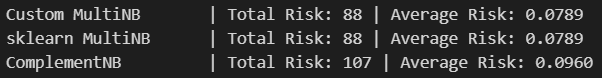
\includegraphics[width=0.75\linewidth]{8.png}
    \caption{نتایج تابع ریسک}
    \label{fig:8}
\end{figure}

بر اساس این داده ها، مشاهده می کنیم که اگرچه مدل complement تعداد بیشتری از پیامک های spam را تشخیص داده است، با این حال هزینه ای که بابت خطاهای دیگر این مدل پرداخت شده است بیشتر بوده و مدل را در معرض ریسک بیشتری قرار می دهد. بنابراین، همچنان در این مسئله مدل Multi پیشنهاد می شود.
\clearpage

\section{پرسش 2}
\href{https://colab.research.google.com/drive/19MJwiHCgJhBfp4knr7LaBVy25tQZMQ3s}{لینک کولب حاوی کدهای این پرسش}



\subsection{آ}

\textbf{توزیع داده‌ها:}

تصاویر در دیتاست MNIST معمولاً مقادیر پیکسل‌هایی از 0 تا 255 دارند که به صورت تقریباً نرمال توزیع می‌شوند.

با استفاده از \lr{StandardScaler}، داده‌ها به گونه‌ای تغییر می‌کنند که میانگین هر ویژگی (هر پیکسل) برابر صفر و انحراف معیار آن برابر یک خواهد شد. این عمل برای مدل‌هایی که به توزیع داده‌ها و نرمال بودن آن‌ها حساس هستند، مانند \lr{SVM} یا \lr{رگرسیون خطی}، مناسب است.

\textbf{الگوریتم‌های استفاده شده:}

اگر قصد استفاده از الگوریتم‌هایی مثل \lr{SVM}، \lr{KNN}، \lr{رگرسیون خطی} یا \lr{شبکه‌های عصبی} را داشته باشیم، \lr{StandardScaler} به دلیل نرمال کردن داده‌ها با توجه به میانگین و انحراف معیار، عملکرد بهتری خواهد داشت.

به‌ویژه برای مدل‌هایی که برای محاسبه فاصله (مثل \lr{KNN}) یا تصمیم‌گیری بر اساس توزیع داده‌ها (مثل \lr{SVM}) طراحی شده‌اند، این نرمال‌سازی بسیار مفید است.

\textbf{چرا MinMaxScaler مناسب نیست؟}

تصاویر \lr{MNIST} معمولاً مقادیر گسترده‌ای از پیکسل‌ها دارند (از 0 تا 255) و نرمال‌سازی آن‌ها به بازه \lr{[0, 1]} با \lr{MinMaxScaler} ممکن است باعث از دست رفتن اطلاعات مربوط به توزیع واقعی داده‌ها شود. به عبارت دیگر، اگر داده‌ها به شدت نامتوازن یا با ویژگی‌هایی با مقادیر بسیار متفاوت باشند، \lr{MinMaxScaler} ممکن است باعث فشرده شدن داده‌ها به بازه کوچکی شود و اطلاعات ارزشمند از بین برود.

\textbf{استفاده در شبکه‌های عصبی}: در صورتی که مدل شما از نوع \lr{شبکه عصبی} باشد، \lr{MinMaxScaler} ممکن است مناسب باشد، ولی در اکثر مواقع با توجه به توزیع نرمال داده‌های \lr{MNIST}، \lr{StandardScaler} بهتر عمل می‌کند.


\subsection{ب}

پس از اعمال کد پایتون نتیجه و خروجی ما مطابق \autoref{fig21} شد.

\begin{figure}[h!]
    \centering
    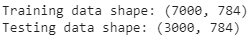
\includegraphics[width=0.5\linewidth]{q2_p1.png}
    \caption{تقسیم داده ها به آموزش و آزمون}
    \label{fig21}
\end{figure}


\subsection{ج}

نتایج ما برای این بخش مطابق زیر است:

\begin{figure}[h!]
    \centering
    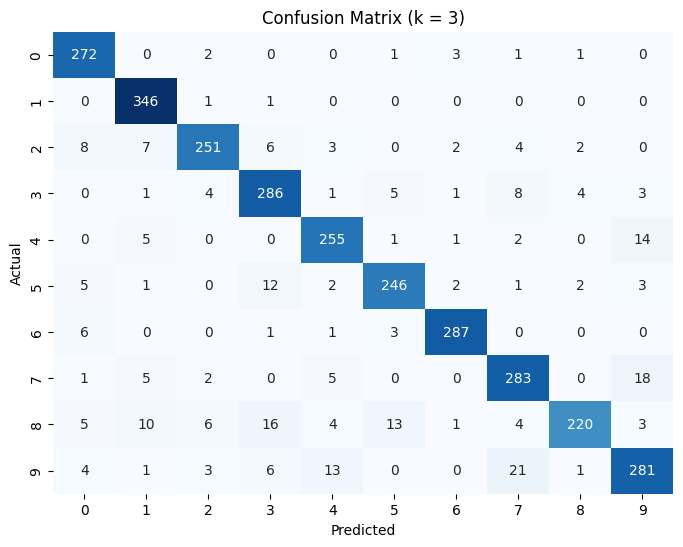
\includegraphics[width=0.6\linewidth]{q2_p31.png}
    \caption{3 = k , :Accuracy 90\%.90}
    \label{fig231}
\end{figure}

\begin{figure}[h!]
    \centering
    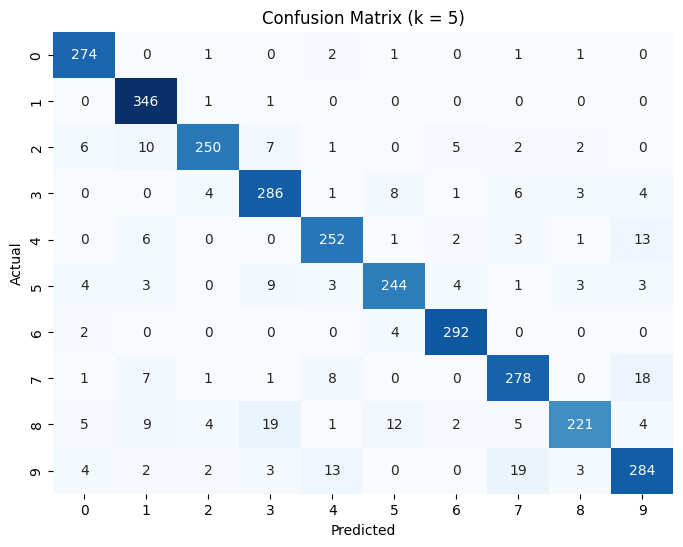
\includegraphics[width=0.6\linewidth]{q2_p32.png}
    \caption{5 = k , :Accuracy 90\%.90}
    \label{fig232}
\end{figure}

\begin{figure}[h!]
    \centering
    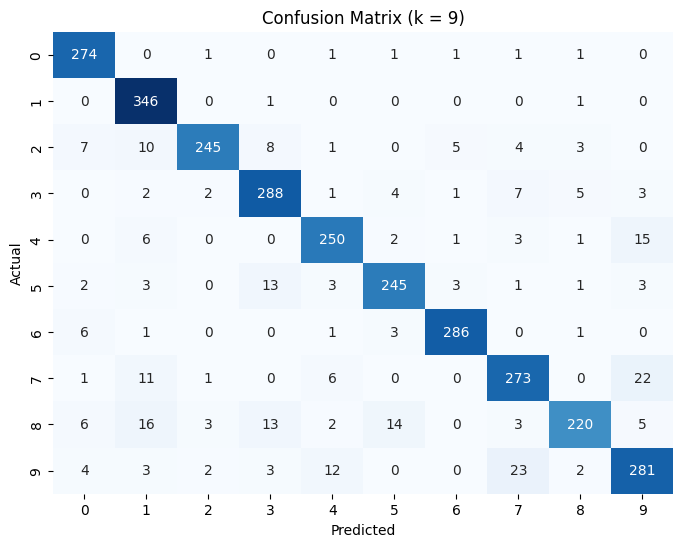
\includegraphics[width=0.6\linewidth]{q2_p33.png}
    \caption{9 = k , :Accuracy 27\%.90}
    \label{fig233}
\end{figure}

حال باید بررسی کنیم که مدل ما برای کدام مقدار k از 1 تا 25 مناسب است. نتایج ما در \autoref{fig234} قابل مشاهده است. طبق این شکل بهترین k برای ما مقدار 3 و 5 می باشد.


\begin{figure}[h!]
    \centering
    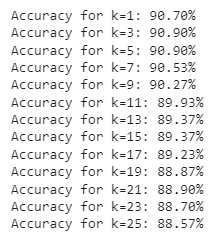
\includegraphics[width=0.4\linewidth]{q2_p34.png}
    \caption{ارزیابی مدل برای k های مختلف}
    \label{fig234}
\end{figure}



\subsection{د}

نمودار خواسته شده از ما برای این بخش در \autoref{fig24} مشاهده می شود. همانطور که دیده می شود بهترین مقدار k برای ما 3 و 5 است.

\begin{figure}[h!]
    \centering
    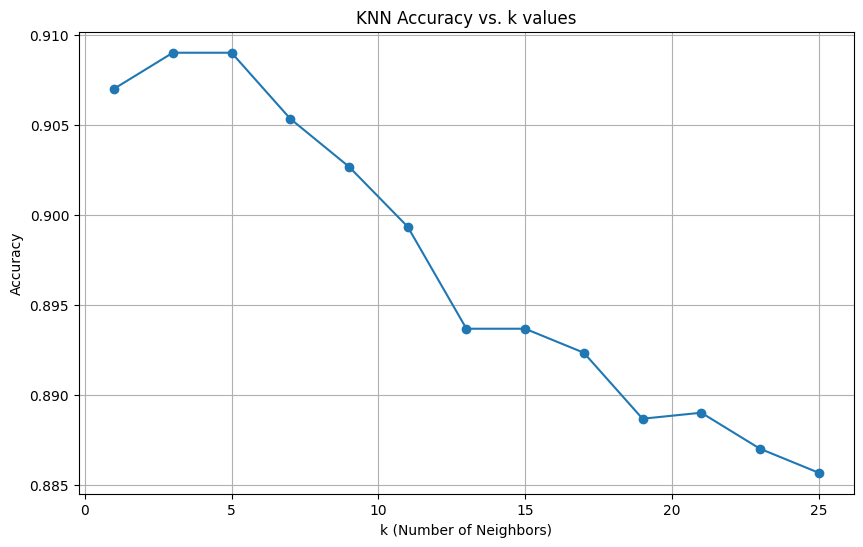
\includegraphics[width=0.6\linewidth]{q2_p4.png}
    \caption{نمودار k های مختلف برای ارزیابی}
    \label{fig24}
\end{figure}


\subsection{ه}


\textbf{ چرا PCA می‌تواند موثر باشد؟}

الگوریتم \lr{K-Nearest Neighbors (KNN)} به شدت به ابعاد بالا حساس است که این پدیده به \textbf{نفرین ابعاد بالا} یا \lr{Curse of Dimensionality} معروف است. در فضای با ابعاد زیاد، فاصله بین داده‌ها کمتر معنی‌دار می‌شود و کارایی مدل‌های یادگیری کاهش می‌یابد.

روش \lr{PCA} با کاهش تعداد ابعاد ویژگی‌ها می‌تواند این مشکل را تا حد زیادی حل کند. مزایای استفاده از \lr{PCA} عبارتند از:

\begin{itemize}
  \item \textbf{فاصله‌ها معنی‌دارتر می‌شوند:} با کاهش ابعاد، داده‌ها در فضایی فشرده‌تر و معنادارتر قرار می‌گیرند، و الگوریتم \lr{KNN} بهتر می‌تواند همسایگان نزدیک را تشخیص دهد.
  \item \textbf{نویز حذف می‌شود:} مؤلفه‌های کم‌اهمیت که معمولاً حامل نویز هستند، حذف می‌شوند و فقط مؤلفه‌های مهم باقی می‌مانند.
  \item \textbf{محاسبات سریع‌تر می‌شوند:} کاهش ابعاد منجر به کاهش بار محاسباتی می‌شود که در حجم بالای داده‌ها بسیار مؤثر است.
\end{itemize}

در نتیجه، با اعمال \lr{PCA} ممکن است مدل \lr{KNN} دقت بالاتری کسب کند و زمان اجرای کمتری نیز داشته باشد.


حال طبق این توضیحات به بررسی سوال می پردازیم. ابتدا مدل را برای مقادیر مختلف مولفه های اصلی بررسی می کنیم. ارزیابی ما در \autoref{fig251} قابل مشاهده است.


\begin{figure}[h!]
    \centering
    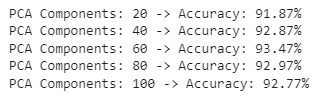
\includegraphics[width=0.6\linewidth]{q2_p51.png}
    \caption{عملکرد مدل برای مولفه های مختلف}
    \label{fig251}
\end{figure}

سپس در \autoref{fig252} نتیجه نمودار را مشاهده می کنیم. مشاهده می شود که بهترین معیار مولفه اصلی 60 می باشد.


\begin{figure}[h!]
    \centering
    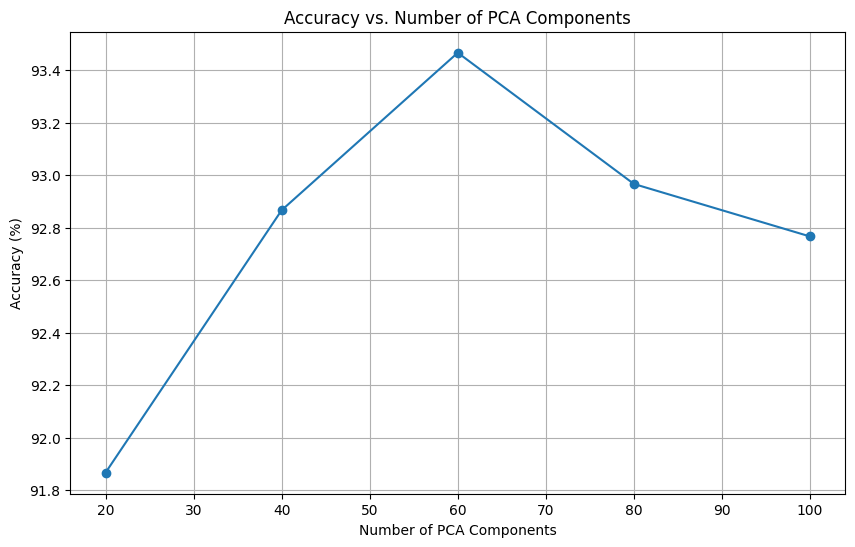
\includegraphics[width=0.6\linewidth]{q2_p52.png}
    \caption{نمودار عملکرد مدل برای مولفه های مختلف}
    \label{fig252}
\end{figure}





\section{پرسش 3}
\href{https://colab.research.google.com/drive/1PsIjMKnh6SxLKSShV9cIGt0ZO9u8hPxs}{لینک کولب حاوی کدهای این پرسش}


\subsection{}

طبق خواسته سوال، 10 سطر اول دیتاست مطابق \autoref{fig31} است.

\begin{figure}[h!]
    \centering
    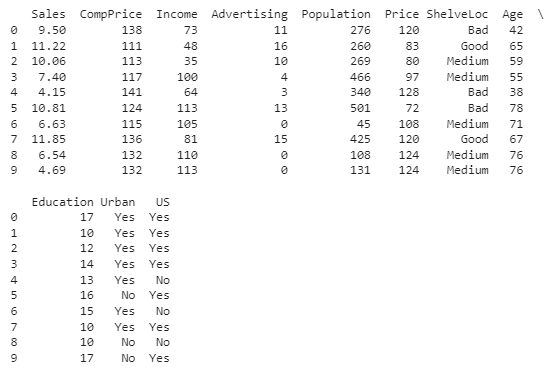
\includegraphics[width=0.9\linewidth]{q4_p1.png}
    \caption{10 سطر اول دیتاست}
    \label{fig31}
\end{figure}


\subsection{پیش پردازش دیتاست}

\subsubsection{بررسی داده های ناقص یا گمشده}

در \autoref{fig321} نتیجه کد بررسی داده های ناقص را مشاهده می کنیم. طبق این نتیجه همانطور که میبینیم دیتاست ما هیچ داده ناقصی ندارد.

\begin{figure}[h!]
    \centering
    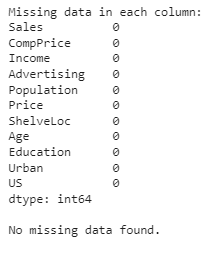
\includegraphics[width=0.6\linewidth]{q3_p21.png}
    \caption{بررسی داده های ناقص در دیتاست}
    \label{fig321}
\end{figure}


\subsubsection{بررسی داده های تکراری}

\textbf{توضیحات درباره داده‌های تکراری:
}

داده‌های تکراری در دیتاست‌ها می‌توانند مشکلات مختلفی برای مدل‌های یادگیری ماشین و تحلیل داده‌ها ایجاد کنند. برخی از این مشکلات عبارتند از:

\begin{itemize}
    \item \textbf{اثرگذاری بیش از حد بر مدل}: داده‌های تکراری باعث می‌شوند که برخی نمونه‌ها وزن زیادی در مدل پیدا کنند، که می‌تواند باعث شود مدل بر اساس این نمونه‌های تکراری بیش از حد تطبیق پیدا کند (Overfitting).
    
    \item \textbf{کاهش دقت مدل}: داده‌های تکراری می‌توانند دقت مدل را کاهش دهند، زیرا مدل ممکن است تمرکز زیادی بر روی داده‌های تکراری بگذارد و از ویژگی‌های دیگر دیتاست به درستی استفاده نکند.
    
    \item \textbf{منحرف کردن تحلیل‌ها}: در تحلیل داده‌ها، داده‌های تکراری می‌توانند نتایج نادرستی ایجاد کنند، به طوری که آنالیزها نمی‌توانند به درستی نتایج مطلوب را ارائه دهند.
    
    \item \textbf{کاهش کارایی}: در مدل‌هایی که به زمان محاسباتی حساس هستند، داده‌های تکراری می‌توانند زمان آموزش و پیش‌بینی را افزایش دهند و در نتیجه کارایی مدل را کاهش دهند.
\end{itemize}



در \autoref{fig321} نتیجه کد بررسی داده های تکراری را مشاهده می کنیم. طبق این نتیجه همانطور که میبینیم دیتاست ما هیچ داده تکراری ندارد.


\begin{figure}[h!]
    \centering
    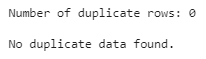
\includegraphics[width=0.6\linewidth]{q3_p22.png}
    \caption{بررسی داده های تکراری در دیتاست}
    \label{fig322}
\end{figure}




\textbf{تبدیل ویژگی‌های دسته‌ای به ویژگی‌های عددی:
}

برای تبدیل ویژگی‌های دسته‌ای (categorical features) به ویژگی‌های عددی (numerical features) در مدل‌های یادگیری ماشین، می‌توان از چند روش مختلف استفاده کرد. متداول‌ترین روش‌ها برای انجام این تبدیل عبارتند از:

\begin{itemize}
    \item \textbf{One-Hot Encoding}: برای ویژگی‌هایی که مقادیر دسته‌ای محدود دارند، استفاده از One-Hot Encoding بسیار رایج است. این روش برای هر مقدار از ویژگی یک ستون جدید ایجاد می‌کند که در آن مقدار "1" برای آن مقدار خاص و "0" برای بقیه مقادیر قرار می‌گیرد.
    
    \item \textbf{Label Encoding}: اگر ویژگی‌ها تنها شامل چند مقدار مختلف باشند (مثلاً "شهر" و "غیرشهر" برای ویژگی محل فروش)، می‌توان از Label Encoding استفاده کرد. این روش هر مقدار را به یک عدد منحصر به فرد تبدیل می‌کند.
\end{itemize}

\textbf{راه‌حل پیشنهادی:
}

برای ویژگی‌های دسته‌ای مانند محل فروش محصول (شهر یا غیرشهر) و فروخته شدن در آمریکا یا خارج از آمریکا، می‌توان از Label Encoding یا One-Hot Encoding استفاده کرد. در صورتی که تعداد مقادیر دسته‌ای محدود باشد (برای مثال فقط دو دسته "شهر" و "غیرشهر" وجود داشته باشد)، استفاده از Label Encoding می‌تواند مناسب باشد. اما برای ویژگی‌هایی که چندین دسته دارند، بهتر است از One-Hot Encoding استفاده کنیم.


در \autoref{fig323} نتیجه کد پایتون برای این بخش را مشاهده می کنیم. طبق توضیحات، داده های بخش US که شامل Yes و No بود به ترتیب به 1 و 0 تبدیل شدند. همچنین داده های ستون Urban نیز که Yes و No بودند به ترتیب به 1 و 0 تبدیل شدند. در نهایت داده های ستون ShelveLoc که شامل Good و Bad و Medium بودند به ترتیب به 1 و 0 و 2 تبدیل شدند. \autoref{fig323} خروجی اصلی و نهایی جدول ما می باشد.

\begin{figure}[h!]
    \centering
    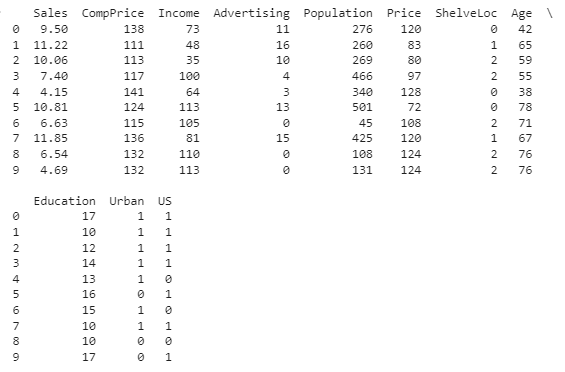
\includegraphics[width=0.8\linewidth]{q3_p23.png}
    \caption{مشاهده 10 سطر اول دیتاست که همه داده های آن عددی هستند.}
    \label{fig323}
\end{figure}


\subsubsection{تبدیل متغیر هدف به متغیر دسته ای}

برای تبدیل متغیر هدف (که در اینجا sales است) به متغیر دسته‌ای (categorical variable)، ابتدا باید میزان فروش (متغیر عددی) را به دسته‌های مختلف تقسیم کنیم. این کار می‌تواند با استفاده از تکنیک‌هایی مانند تقسیم بازه‌ای (binning) انجام شود.


\textbf{پیشنهاد بازه‌ها برای دسته‌بندی:}

با توجه به میانگین 49.7، می‌توانیم \texttt{sales} را به دسته‌های زیر تقسیم کنیم:

\begin{itemize}
    \item \textbf{کم فروش (Low Sales)}: مقادیری که کمتر از میانگین هستند.
    \item \textbf{متوسط فروش (Medium Sales)}: مقادیری که در نزدیکی میانگین قرار دارند.
    \item \textbf{زیاد فروش (High Sales)}: مقادیری که بیشتر از میانگین هستند.
\end{itemize}

برای انجام این کار، پیشنهاد می‌شود که محدوده‌ها را بر اساس درصدی از میانگین و دامنه داده‌ها تنظیم کنیم.

\textbf{پیشنهاد بازه‌ها:}

\begin{itemize}
    \item \textbf{کم فروش (Low)}: \texttt{sales} کمتر از 5.4
    \item \textbf{متوسط فروش (Medium)}: \texttt{sales} بین 5.4 و 10
    \item \textbf{زیاد فروش (High)}: \texttt{sales} بیشتر از 10
\end{itemize}

سپس در \autoref{fig324} 10 سطر اول داده های فروش و داده های دسته بندی شده را مشاهده می کنیم.

\begin{figure}[h!]
    \centering
    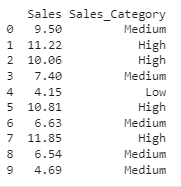
\includegraphics[width=0.6\linewidth]{q3_p24.png}
    \caption{مشاهده 10 سطر اول دیتاست داده های فروش و داده های دسته شده }
    \label{fig324}
\end{figure}

در نهایت این داده های متنی را به داده های عددی تبدیل می کنیم. بدین صورت که Low به 0، Medium به 1 و High به 2 تبدیل شدند. 10 سطر اول ما در \autoref{fig3241} قابل مشاهده است.

\begin{figure}[h!]
    \centering
    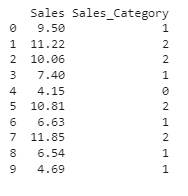
\includegraphics[width=0.6\linewidth]{q3_p241.png}
    \caption{مشاهده 10 سطر اول دیتاست داده های فروش و داده های دسته شده تبدیل شده به داده های عددی }
    \label{fig3241}
\end{figure}


\subsubsection{ماتریس همبستگی}

ماتریس همبستگی ما مطابق \autoref{fig325} می باشد.

\begin{figure}[h!]
    \centering
    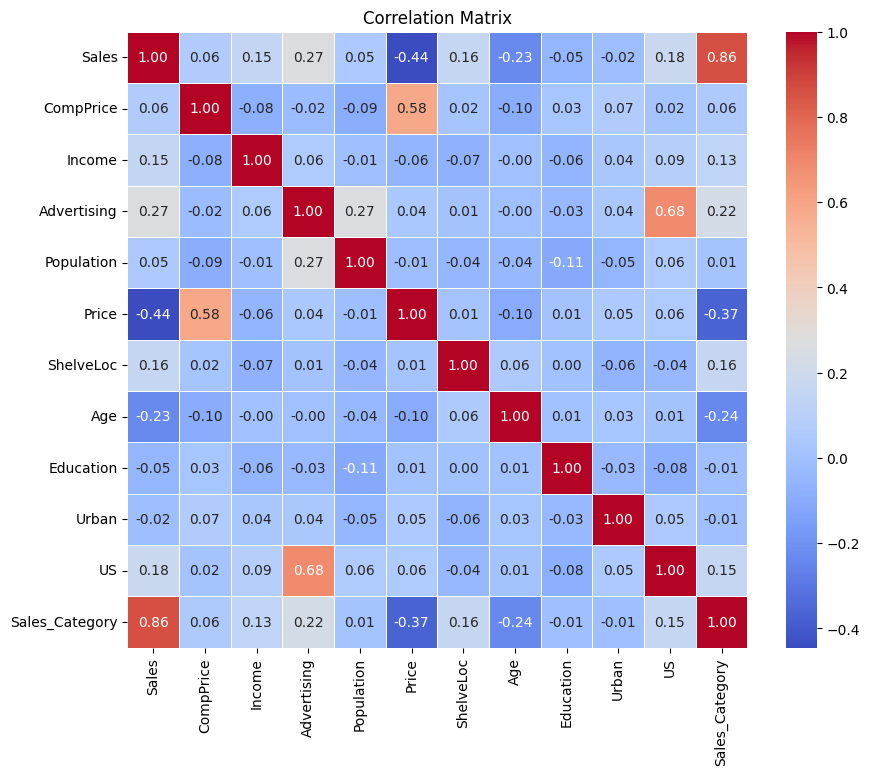
\includegraphics[width=0.8\linewidth]{q3_p25.png}
    \caption{بررسی ماتریس همبستگی}
    \label{fig325}
\end{figure}


\subsubsection{بررسی همبستگی ها}

در \autoref{fig326} ما ترتیب میان بیشترین همبستگی ما دسته بندی Sales را داریم. طبق این شکل بیشترین میزان همبستگی این دسته با Sales ، Advertising ، ShelveLoc ، US و Income می باشد. همچنین همبستگی میان CompPrice با Price و US با Advertising نیز زیاد و قابل توجه است.

\begin{figure}[h!]
    \centering
    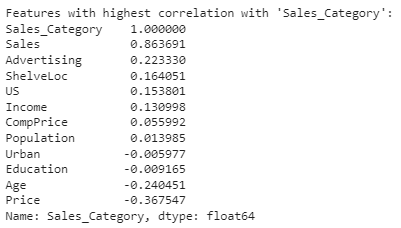
\includegraphics[width=0.6\linewidth]{q3_p26.png}
    \caption{بررسی ارتباط میان همبستگی ها}
    \label{fig326}
\end{figure}


\subsection{محاسبه آنتروپی داده ها}


آنتروپی (Entropy) یک معیار برای اندازه‌گیری عدم‌قطعیت یا بی‌نظمی در داده‌ها است. در مدل‌های یادگیری ماشین، محاسبه آنتروپی می‌تواند به ما کمک کند تا میزان اطلاعات یا عدم‌قطعیت موجود در یک مجموعه داده را ارزیابی کنیم.

برای محاسبه آنتروپی یک مجموعه از داده‌ها، از فرمول زیر استفاده می‌کنیم:

\[
\text{Entropy}(S) = - \sum_{i=1}^{n} p_i \cdot \log_2(p_i)
\]

که در آن:
\begin{itemize}
    \item \( p_i \) احتمال وقوع هر برچسب (label) است.
    \item \( n \) تعداد کلاس‌ها یا مقادیر مختلف است.
\end{itemize}

در کد زیر، ابتدا آنتروپی برای ویژگی \texttt{Sales} و سپس برای \texttt{Sales\_Category} محاسبه می‌شود.

\textbf{کد محاسبه آنتروپی:}

در ابتدا تابع \texttt{calculate\_entropy} به این شکل تعریف می‌شود:

\begin{lstlisting}[language=Python]
def calculate_entropy(y):
    # Count the frequency of each unique label in the array y
    unique, counts = np.unique(y, return_counts=True)

    # Calculate probabilities of each unique label
    probabilities = counts / len(y)

    # Calculate entropy using the formula: -sum(p * log2(p))
    entropy = -np.sum(probabilities * np.log2(probabilities))

    return entropy
\end{lstlisting}

\textbf{توضیحات کد:}
\begin{itemize}
    \item ابتدا با استفاده از \texttt{np.unique} تعداد وقوع هر برچسب یا کلاس در آرایه \texttt{y} شمارش می‌شود.
    \item سپس احتمال وقوع هر برچسب با تقسیم تعداد وقوع‌ها بر تعداد کل داده‌ها محاسبه می‌شود.
    \item در نهایت آنتروپی با استفاده از فرمول \(- \sum p_i \cdot \log_2(p_i)\) محاسبه می‌شود.
\end{itemize}

برای محاسبه آنتروپی ویژگی‌های \texttt{Sales} و \texttt{Sales\_Category}، ابتدا باید ویژگی \texttt{Sales} را به دسته‌ها تقسیم کنیم. سپس آنتروپی برای هر یک محاسبه می‌شود.

\textbf{محاسبه آنتروپی برای ویژگی‌های مختلف:}

\begin{lstlisting}[language=Python]
# Calculate entropy for 'sales' (by converting to categories)
# We need to bin 'sales' into categories first
sales_bins = pd.cut(data['Sales'], bins=bins, labels=labels, right=False)
sales_entropy = calculate_entropy(sales_bins)

# Calculate entropy for 'Sales_Category'
sales_category_entropy = calculate_entropy(data['Sales_Category'])

# Display the results
print(f"Entropy of 'Sales': {sales_entropy}")
print(f"Entropy of 'Sales_Category': {sales_category_entropy}")
\end{lstlisting}

\textbf{توضیحات کد:}

\begin{itemize}
    \item در ابتدا ویژگی \texttt{Sales} به دسته‌هایی مانند "کم فروش"، "متوسط فروش" و "زیاد فروش" تقسیم می‌شود. این کار با استفاده از تابع \texttt{pd.cut} انجام می‌شود که بازه‌های مشخصی برای داده‌ها تعریف می‌کند.
    \item سپس آنتروپی برای ویژگی \texttt{Sales} و \texttt{Sales\_Category} با استفاده از تابع \texttt{calculate\_entropy} محاسبه می‌شود.
    \item در نهایت، مقادیر آنتروپی برای هر یک از ویژگی‌ها نمایش داده می‌شود.
\end{itemize}

\textbf{نتیجه‌گیری:
}

آنتروپی محاسبه‌شده برای هر ویژگی نشان‌دهنده میزان عدم‌قطعیت یا پیچیدگی موجود در داده‌ها است. آنتروپی بالا نشان‌دهنده توزیع یکنواخت و متنوع در داده‌ها است، در حالی که آنتروپی پایین نشان‌دهنده این است که داده‌ها بیشتر به یک یا چند کلاس خاص متمایل هستند.

در ضمن میزان آنتروپی برای داده های هدف ما 2414351448162364.1 شد.

\subsection{محاسبه Gain Information}


در این بخش، هدف محاسبه \textbf{Gain Information} برای ویژگی \texttt{Sales\_Category} است. \textbf{Gain Information} به ما کمک می‌کند تا بدانیم یک ویژگی چقدر می‌تواند اطلاعات جدید به مدل اضافه کند. این معیار معمولاً در الگوریتم‌های درخت تصمیم برای انتخاب ویژگی‌ها استفاده می‌شود.

فرمول محاسبه \textbf{Gain Information} به شرح زیر است:

\[
\text{Gain Information} = \text{Entropy}(parent) - \sum_{i} \left( \frac{|S_i|}{|S|} \cdot \text{Entropy}(S_i) \right)
\]

که در آن:
\begin{itemize}
    \item \( \text{Entropy}(parent) \) آنتروپی مجموعه والد است.
    \item \( \frac{|S_i|}{|S|} \) وزن هر زیرمجموعه \( S_i \) است.
    \item \( \text{Entropy}(S_i) \) آنتروپی هر زیرمجموعه \( S_i \) است.
\end{itemize}

در کد زیر، ابتدا آنتروپی مجموعه والد (\texttt{parent}) و سپس آنتروپی زیرمجموعه‌ها (یعنی \texttt{children}) محاسبه می‌شود. در نهایت، \textbf{Information Gain} محاسبه می‌شود.

\textbf{کد محاسبه Gain: Information}

\begin{lstlisting}[language=Python]
def info_gain(parent, children):
    # Calculate the entropy of the parent (the whole dataset)
    parent_entropy = calculate_entropy(parent)

    # Calculate the weighted entropy of the children
    total_size = len(parent)
    weighted_entropy = 0
    for child in children:
        child_entropy = calculate_entropy(child)
        weighted_entropy += (len(child) / total_size) * child_entropy

    # Calculate Information Gain
    gain = parent_entropy - weighted_entropy
    return gain
\end{lstlisting}

\textbf{توضیحات کد:}

\begin{itemize}
    \item تابع \texttt{info\_gain} به محاسبه \textbf{Gain Information} بین مجموعه والد و زیرمجموعه‌ها پرداخته است.
    \item ابتدا آنتروپی مجموعه والد با استفاده از تابع \texttt{calculate\_entropy} محاسبه می‌شود.
    \item سپس آنتروپی هر زیرمجموعه (\texttt{children}) محاسبه و به صورت وزنی جمع می‌شود.
    \item در نهایت، \textbf{Gain Information} با تفاضل آنتروپی والد و آنتروپی وزنی زیرمجموعه‌ها محاسبه می‌شود.
\end{itemize}

\textbf{محاسبه Gain Information برای ویژگی‌ها:}

در این بخش، \textbf{Gain Information} برای ویژگی \texttt{Sales\_Category} محاسبه می‌شود. ابتدا ویژگی \texttt{Sales} به دسته‌های مختلف تقسیم می‌شود، سپس \textbf{Gain Information} محاسبه می‌شود.

\begin{lstlisting}[language=Python]
parent = data['Sales_Category']  # Parent is the 'Sales_Category'
children = [data['Sales'][sales_bins == 'Low'],  # First child subset (Low)
            data['Sales'][sales_bins == 'Medium'],  # Second child subset (Medium)
            data['Sales'][sales_bins == 'High']]  # Third child subset (High)

# Calculate Information Gain for 'Sales_Category'
sales_gain = info_gain(parent, children)

# Display the results
print(f"Information Gain for 'Sales_Category': {sales_gain}")
\end{lstlisting}

\textbf{توضیحات کد:}

\begin{itemize}
    \item در این قسمت، ویژگی \texttt{Sales\_Category} به عنوان مجموعه والد (\texttt{parent}) در نظر گرفته می‌شود.
    \item ویژگی \texttt{Sales} به سه دسته "کم فروش" (\texttt{Low})، "متوسط فروش" (\texttt{Medium}) و "زیاد فروش" (\texttt{High}) تقسیم می‌شود.
    \item پس از تقسیم داده‌ها، \textbf{Gain Information} برای \texttt{Sales\_Category} محاسبه می‌شود.
    \item در نهایت، مقدار \textbf{Gain Information} برای \texttt{Sales\_Category} نمایش داده می‌شود.
\end{itemize}

در نهایت Gain Information برای تابع هدف برابر با 820888150098982.5- شد.

\subsection{درخت تصمیم}
\subsubsection{Pruning}
مدل طبقه بندی درخت تصمیم قادر است با ایجاد تعداد شاخه های زیاد، در نهایت به دیتاست فیت بشود. با این حال، در صورتی که عمق مشخصی برای شاخه ها تعیین نشود، به راحتی به بیش برازش منجر می شود تا آنجا که به ازای هر نمونه، یک شاخه به وجود می آید و در واقعیت، یک $lookup table$ به دست می آید.
برای جلوگیری از این رخداد، از روش های Pruning برای محدود کردن درخت و کسب $generalization$ صورت می گیرد.
این فرایند، به دو صورت انجام می شود.
\begin{enumerate}
    \item $Pre Pruning (Early Stopinng)$: 

    در این روش، مانند اکثر مدل های یادگیری ماشین، میزان آستانه ای از پیش برای درخت تعیین می شود. این آستانه می تواند بر عمق درخت، تعداد نمونه های موجود در هر شاخه، باشد.بنابراین، در این روش مدل در حین یادگیری، از اورفیت شدن به داده ها جلوگیری می کند.

    \item $Post Pruning$

    در این روش، ابتدا بدون اعمال محدودیت بر شاخه های درخت، مدل در بهترین حالت آموزش می بیند. بدیهی است که در  فرایند آموزش، مدل به طور کامل به داده های آموزشی اورفیت می شود. پس از آن، با حذف شاخه هایی که در عملکرد مدل تاثیر کمتری دارند، در راستای generalize کردن مدل پیش می رویم. معیار های انتخاب و حذف شاخه ها در این روش متفوت است که از آن جمله می توان به  $Cost Complecity$ اشاره کرد.
    
\end{enumerate}

\subsubsection{آموزش مدل با Grid search}
برای آموزش مدل درخت تصیم، ابتدا دیتافریم های ویژگی ها و برچسب ها را جدا کرده و سپس با اعمال دستور TrainTestSplit، آنها را به داده های آموزشی و تستی تقسیم می کنیم. 

در گام بعد، یک مدل درخت تصمیم تعریف می شود. با این حال، تنظیم هایپرپارامتر های این مدل نیز باید در فرایند آموزش های مکرر بهینه سازی شود. در اینجا، از روش GridSearchCV برای بهینه کردن مدل استفاده می کنیم.

برای این منظور، لازم است مقادیری که به ازای آنها می خواهیم عملکرد مدل را بررسی کنیم برای این روش تعریف کنیم. برای آموزش درخت تصمیم در این تمرین، از گزینه های زیر برای آموزش درخت استفاده شده است:
\begin{table}[h!]
\centering
\begin{tabular}{|l|l|}
\hline
\textbf{Parameter} & \textbf{Values} \\
\hline
\texttt{criterion} & \{``gini'', ``entropy''\} \\
\texttt{max\_depth} & \{None, 10, 20, 30\} \\
\texttt{min\_samples\_split} & \{2, 5, 10\} \\
\texttt{min\_samples\_leaf} & \{1, 2, 4\} \\
\texttt{max\_features} & \{None, ``auto'', ``sqrt'', ``log2''\} \\
\hline
\end{tabular}
\caption{Grid of hyperparameters used in GridSearchCV}
\label{tab:param_grid}
\end{table}

پس از اجرای این کد بر روی مدل و ارزیابی عملکرد مدل ها با پارامترهای مختلف، در نهایت پاسخ بهینه به صورت زیر به دست می آید.
\begin{table}[h!]
\centering
\begin{tabular}{|l|l|}
\hline
\textbf{Parameter} & \textbf{Selected Value} \\
\hline
\texttt{max\_depth} & 10 \\
\texttt{max\_features} & ``sqrt'' \\
\texttt{min\_samples\_leaf} & 4 \\
\texttt{min\_samples\_split} & 10 \\
\texttt{Best Cross-validation Score} & $0.6642857142857144$ \\
\hline
\end{tabular}
\caption{Best hyperparameters found via GridSearchCV}
\label{tab:best_params}
\end{table}

در توضیح نحوه ی عملکرد روش GridSearch 
می توان گفت این روش مشخصا برای تعیین بهینه ترین ترکیب از هایپرپارامتر ها استفاده می شود. برای بهینه سازی، به ازای تمام ترکیبات ممکن از هایپرپارامتر هایی که برای این مدل فرض می شود، با استفاده از روش k-fold مدل هایی را بر داده های Train آموزش می دهد. در صورتی که مقدار k برابر 5 در نظر گرفته شده باشد، هر بار 4 قسمت از 5 قسمت داده های آموزشی را به آموزش اختصاص داده و بخش پنجم را به عنوان داده ی تست در نظر می گیرد و در نتیجه به ازای هر ترکیب از هایپر پارامتر ها، در نهایت 5 مدل آموزش داده و برای هر یک امتیازی به محاسبه می کند. در نهایت، میانگین امتیاز های این 5 مدل به ازای هایپرپارامتر های مشخص به عنوان امتیاز نهایی این ترکیب ها ذخیره می شود. 

این فرایند برای تمام ترکیب ها انجام شده و در نهایت، ترکیبی که بالاترین امتیاز را داشته باشد به عنوان بهترین تخمین گر گزارش می شود.

با استفاده از این مدل انتخاب شده، نهایتا عملکرد آن را بر داده های تست می سنجیم که در اینجا دقتی برابر با 65\% به دست آمده است.

\subsubsection{رسم درخت تصمیم}

پس از آموزش مدل، با استفاده از دستور plot\_tree و تنظیم بعضی مقادیر برای قرارگیری درست شاخه های درخت برای نمایش بهتر، در نهایت درخت تصمیم حاصل مانند شکل نمایش داده می شود.

\begin{figure}
    \centering
    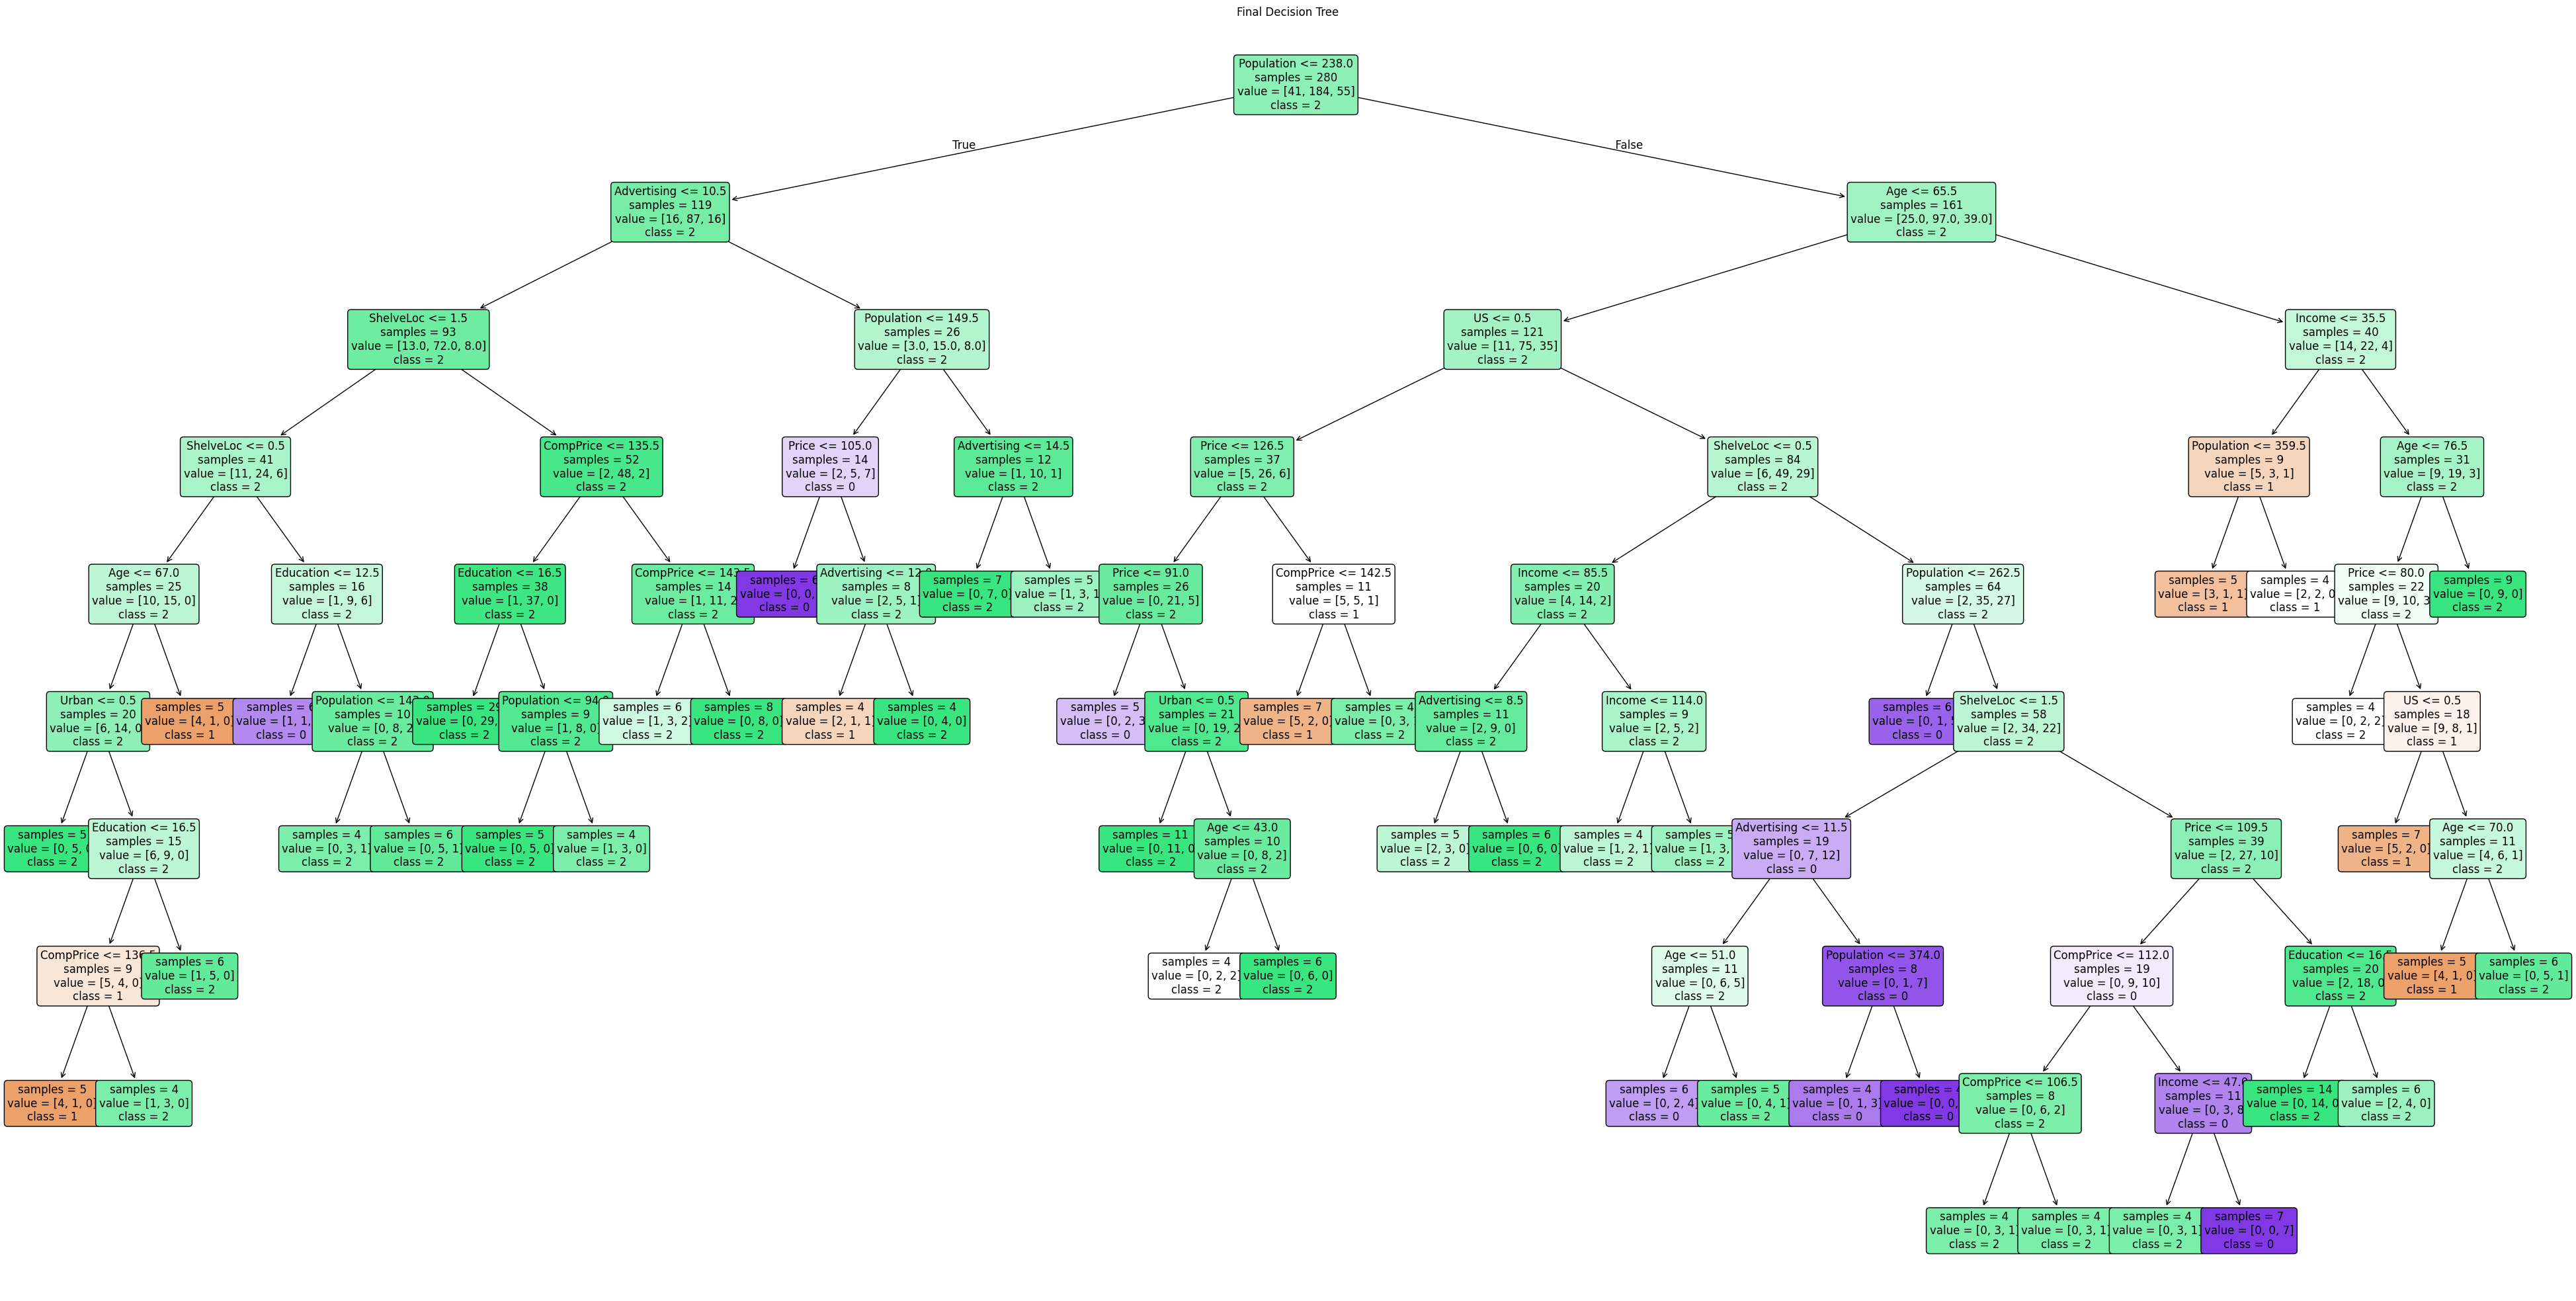
\includegraphics[width=1\linewidth]{Dt.png}
    \caption{درخت تصمیم}
    \label{fig:dt}
\end{figure}

\subsubsection{بررسی Overfit و Underfit}
برای بررسی آنکه آیا مدل به داده های آموزشی بیش برازش شده است یا خبر، در هر مدل دقت مدل را بر روی داده های آموزش و آزمایشی اندازه گیری می کنیم. برای دو مدل فوق نتایج به صورت زیر خواهد بود:
\begin{table}[h!]
\centering
\begin{tabular}{|l|c|c|}
\hline
\textbf{Model} & \textbf{Training Accuracy} & \textbf{Test Accuracy} \\
\hline
Initial Decision Tree & $1.0000$ & $0.5583$ \\
Best Model (GridSearchCV) & $0.8286$ & $0.7000$ \\
\hline
\end{tabular}
\caption{Accuracy of models}
\label{tab:model_accuracy}
\end{table}
بر اساس این مقادیر می توانیم به وضوح مشاهده کنیم که درخت تصمیم آموزش داده شده به  داده های آموزشی اورفیت شده و در آزمایش بر روی این داده ها، دقت 100\% دارد. با این حال، مشاهده می شود که دقت این مدل بر داده های آزمایشی تنها 55\% بوده که یعنی به مقدار کافی generalized نیست.

مدل دیگر که توسط GridSearch انتخاب شده است، با 82\% دقت در داده های آموزشی و 70\% در داده های آزمایشی، عملکرد بهتری را نشان می دهد و اورفیت نیز نشده است.

می توان مشاهده کرد که درخت تصمیم چنان که انتظار می رود، می تواند در نهایت به داده های آموزشی اورفیت شود. برای جلوگیری از این موضوع، می توان از روش های Prouning که بالاتر توضیح داده شد برای حذف شاخه های اضافه که تاثیر چندانی بر عملکرد مدل ندارند استفاده کرد تا مدل هر چه بیشتر فراگیر و generalized شود.

\subsubsection{گزارش عملکرد مدل ها}
در بخش پایانی، گزارش طبقه بندی برای مدل های آموزش داده شده را قرار می دهیم.

\begin{itemize}
    \item گزارش طبقه بندی درخت تصمیم

\begin{itemize}
    \item Accuracy: $0.5583$
    \item Weighted Precision: $0.6212$
    \item Weighted Recall: $0.5583$
    \item Weighted F1-score: $0.5778$
\end{itemize}

\vspace{0.5em}

\begin{table}[h!]
\centering
\begin{tabular}{|c|c|c|c|c|}
\hline
\textbf{Class} & \textbf{Precision} & \textbf{Recall} & \textbf{F1-score} & \textbf{Support} \\
\hline
0 & $0.22$ & $0.31$ & $0.26$ & $13$ \\
1 & $0.75$ & $0.59$ & $0.66$ & $83$ \\
2 & $0.38$ & $0.58$ & $0.46$ & $24$ \\
\hline
\textbf{Accuracy} & \multicolumn{4}{c|}{$0.5583$} \\
\textbf{Macro avg} & $0.45$ & $0.49$ & $0.46$ & $120$ \\
\textbf{Weighted avg} & $0.62$ & $0.56$ & $0.58$ & $120$ \\
\hline
\end{tabular}
\caption{گزارش طبقه‌بندی مدل درخت تصمیم (Best Model)}
\label{tab:dt_classification_report_best}
\end{table}



\begin{figure}
    \centering
    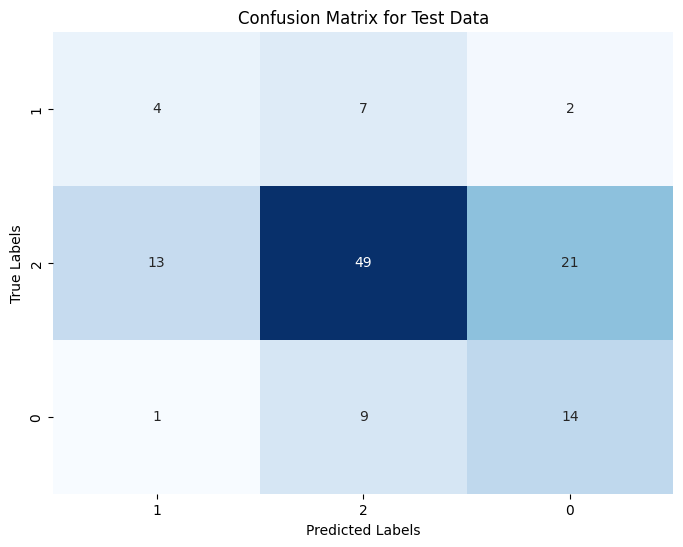
\includegraphics[width=0.75\linewidth]{DT_Confusion.png}
    \caption{ماتریس در هم ریختگی درخت تصمیم}
    \label{fig:enter-label}
\end{figure}
\clearpage

\item گزارش طبقه بندی GridSearch

\begin{itemize}
    \item Accuracy: $0.7000$
    \item Weighted Precision: $0.6823$
    \item Weighted Recall: $0.7000$
    \item Weighted F1-score: $0.6814$
\end{itemize}

\vspace{0.5em}

\begin{table}[h!]
\centering
\begin{tabular}{|c|c|c|c|c|}
\hline
\textbf{Class} & \textbf{Precision} & \textbf{Recall} & \textbf{F1-score} & \textbf{Support} \\
\hline
0 & $0.27$ & $0.23$ & $0.25$ & $13$ \\
1 & $0.76$ & $0.87$ & $0.81$ & $83$ \\
2 & $0.64$ & $0.38$ & $0.47$ & $24$ \\
\hline
\textbf{Accuracy} & \multicolumn{4}{c|}{$0.7000$} \\
\textbf{Macro avg} & $0.56$ & $0.49$ & $0.51$ & $120$ \\
\textbf{Weighted avg} & $0.68$ & $0.70$ & $0.68$ & $120$ \\
\hline
\end{tabular}
\caption{Classification Report for Decision Tree Model}
\label{tab:dt_classification_report}
\end{table}

\begin{figure}
    \centering
    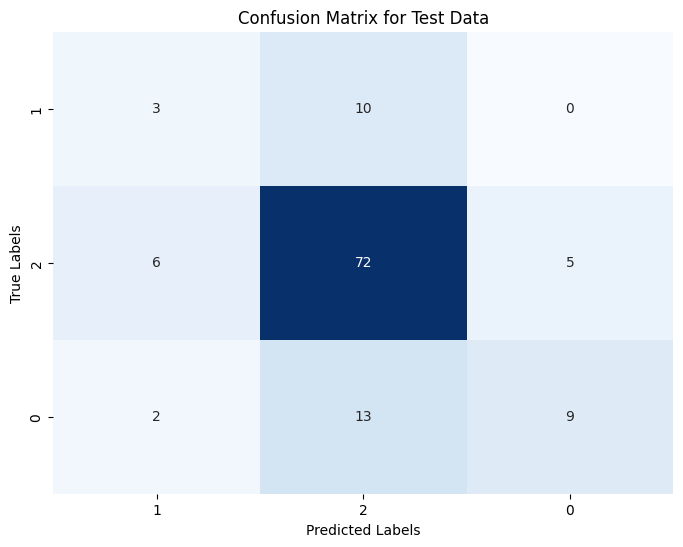
\includegraphics[width=0.75\linewidth]{GridReport.png}
    \caption{ماتریس در هم ریختگی GridSearch}
    \label{fig:enter-label}
\end{figure}
\end{itemize}

در مقایسه ی رفتار این دو مدل مشاهده می کنیم که مدل ردخت تصمیم به داده های آموزشی اورفیت شده است و در مواجهه با داده های دیده نشده ی آزمایشی، در مقابل مدل GridSearch با اختلافی در حدود 14\% عملکرد ضعیف تری دارد.
با نگاه دقیق تر به ماتریس های به هم ریختگی متوجه می شویم که هر دو مدل در تعیین وضعیت داده های کلاس 2 که معادل داده های نرمال و میانه هستند عملکرد بهتری دارند. این اتفاق می تواند ناشی از نامتوازن بودن دیتاست در تعداد داده ها باشد. با این حال، مشاهده می کنیم که هر دو مدل در تعیین داده های کلاس 0 عملکرد ضعیفی دارند. در مورد کلاس 0 نیز می توانیم مشاهده کنیم که اندکی عملکرد مدل ها بهتر است، با این حال در موارد زیادی داده های این کلاس به اشتباه برچسب کلاس 2 را به خود گرفته اند. 

به عنوان نتیجه گیری می توان گفت مدل GridSearch مدل جامع تری است و می تواند داده های غالب سیستم را که مربوط به کلاس 2 هستند بهتر طبقه بندی کند. و مدل درخت تصمیم به دلیل اورفیت شدن، در داده های واقعی که هنوز ندیده است عملکرد ضعیف تری دارد.

\end{document}

